
\resetcounters

\markboth{Michel et al.}{A New Web Interface for Saada}

\title{A New Web Interface for \ssindex{databases!tools!Saada}Saada}
\author{Laurent~Michel,$^1$ Gr\'egory~Mantelet,$^2$ Christian~Motch,$^1$ and Emilie~Werner$^1$
\affil{$^1$Observatoire Astronomique, 11 Rue de l'Universit\'e, 67000 Strasbourg, France}
\affil{$^2$CDS, 11 Rue de l'Universi\'te, 67000 Strasbourg, France}}

\aindex{Michel, L.}
\aindex{Mantelet, G.}
\aindex{Motch, C.}
\aindex{Werner, E.}

\begin{abstract}
\ssindex{databases!tools!Saada}Saada\ooindex{Saada, ascl:1111.003} transforms a set of heterogeneous \ssindex{data formats!FITS}FITS files or \ssindex{data formats!VOTable}VOTables of various categories (images, tables, spectra, etc.) in a powerful database deployed on the Web without writing code. \ssindex{databases!tools!Saada}Saada can mix data of various categories in multiple collections. Data collections can each be linked to others, making relevant browsing paths and allowing data-\ssindex{data!mining}mining oriented queries. \ssindex{databases!tools!Saada}Saada supports 4\ssindex{Virtual Observatory(VO)} VO services (spectra, images, sources and \ssindex{protocols!TAP}TAP) . Data collections can be published immediately after the deployment of the Web interface. The poster presents the new the administration interface (beta) coming with \ssindex{databases!tools!Saada}Saada\ooindex{Saada, ascl:1111.003} databases. This application is much more user-friendly. It also makes the publication of data collections into the\ssindex{Virtual Observatory(VO)} VO very easy.
\end{abstract}

\section{Introduction}
All databases generated by \ssindex{databases!tools!Saada}Saada\ooindex{Saada, ascl:1111.003} \citep{SAADA} have the same hierarchical data model. Data are organized in heterogeneous collections which can be interconnected to others by relationships. Building an administration interface for such a data set remains challenging. The difficulty here is that any action must be associated with only one data set. The binding between a data set and the active function must remain clear enough to avoid users making serious mistakes. The other guideline of this development was to help users to publish their data in the\ssindex{Virtual Observatory(VO)} VO registry.

\begin{figure}[!ht]
	\begin{center}
		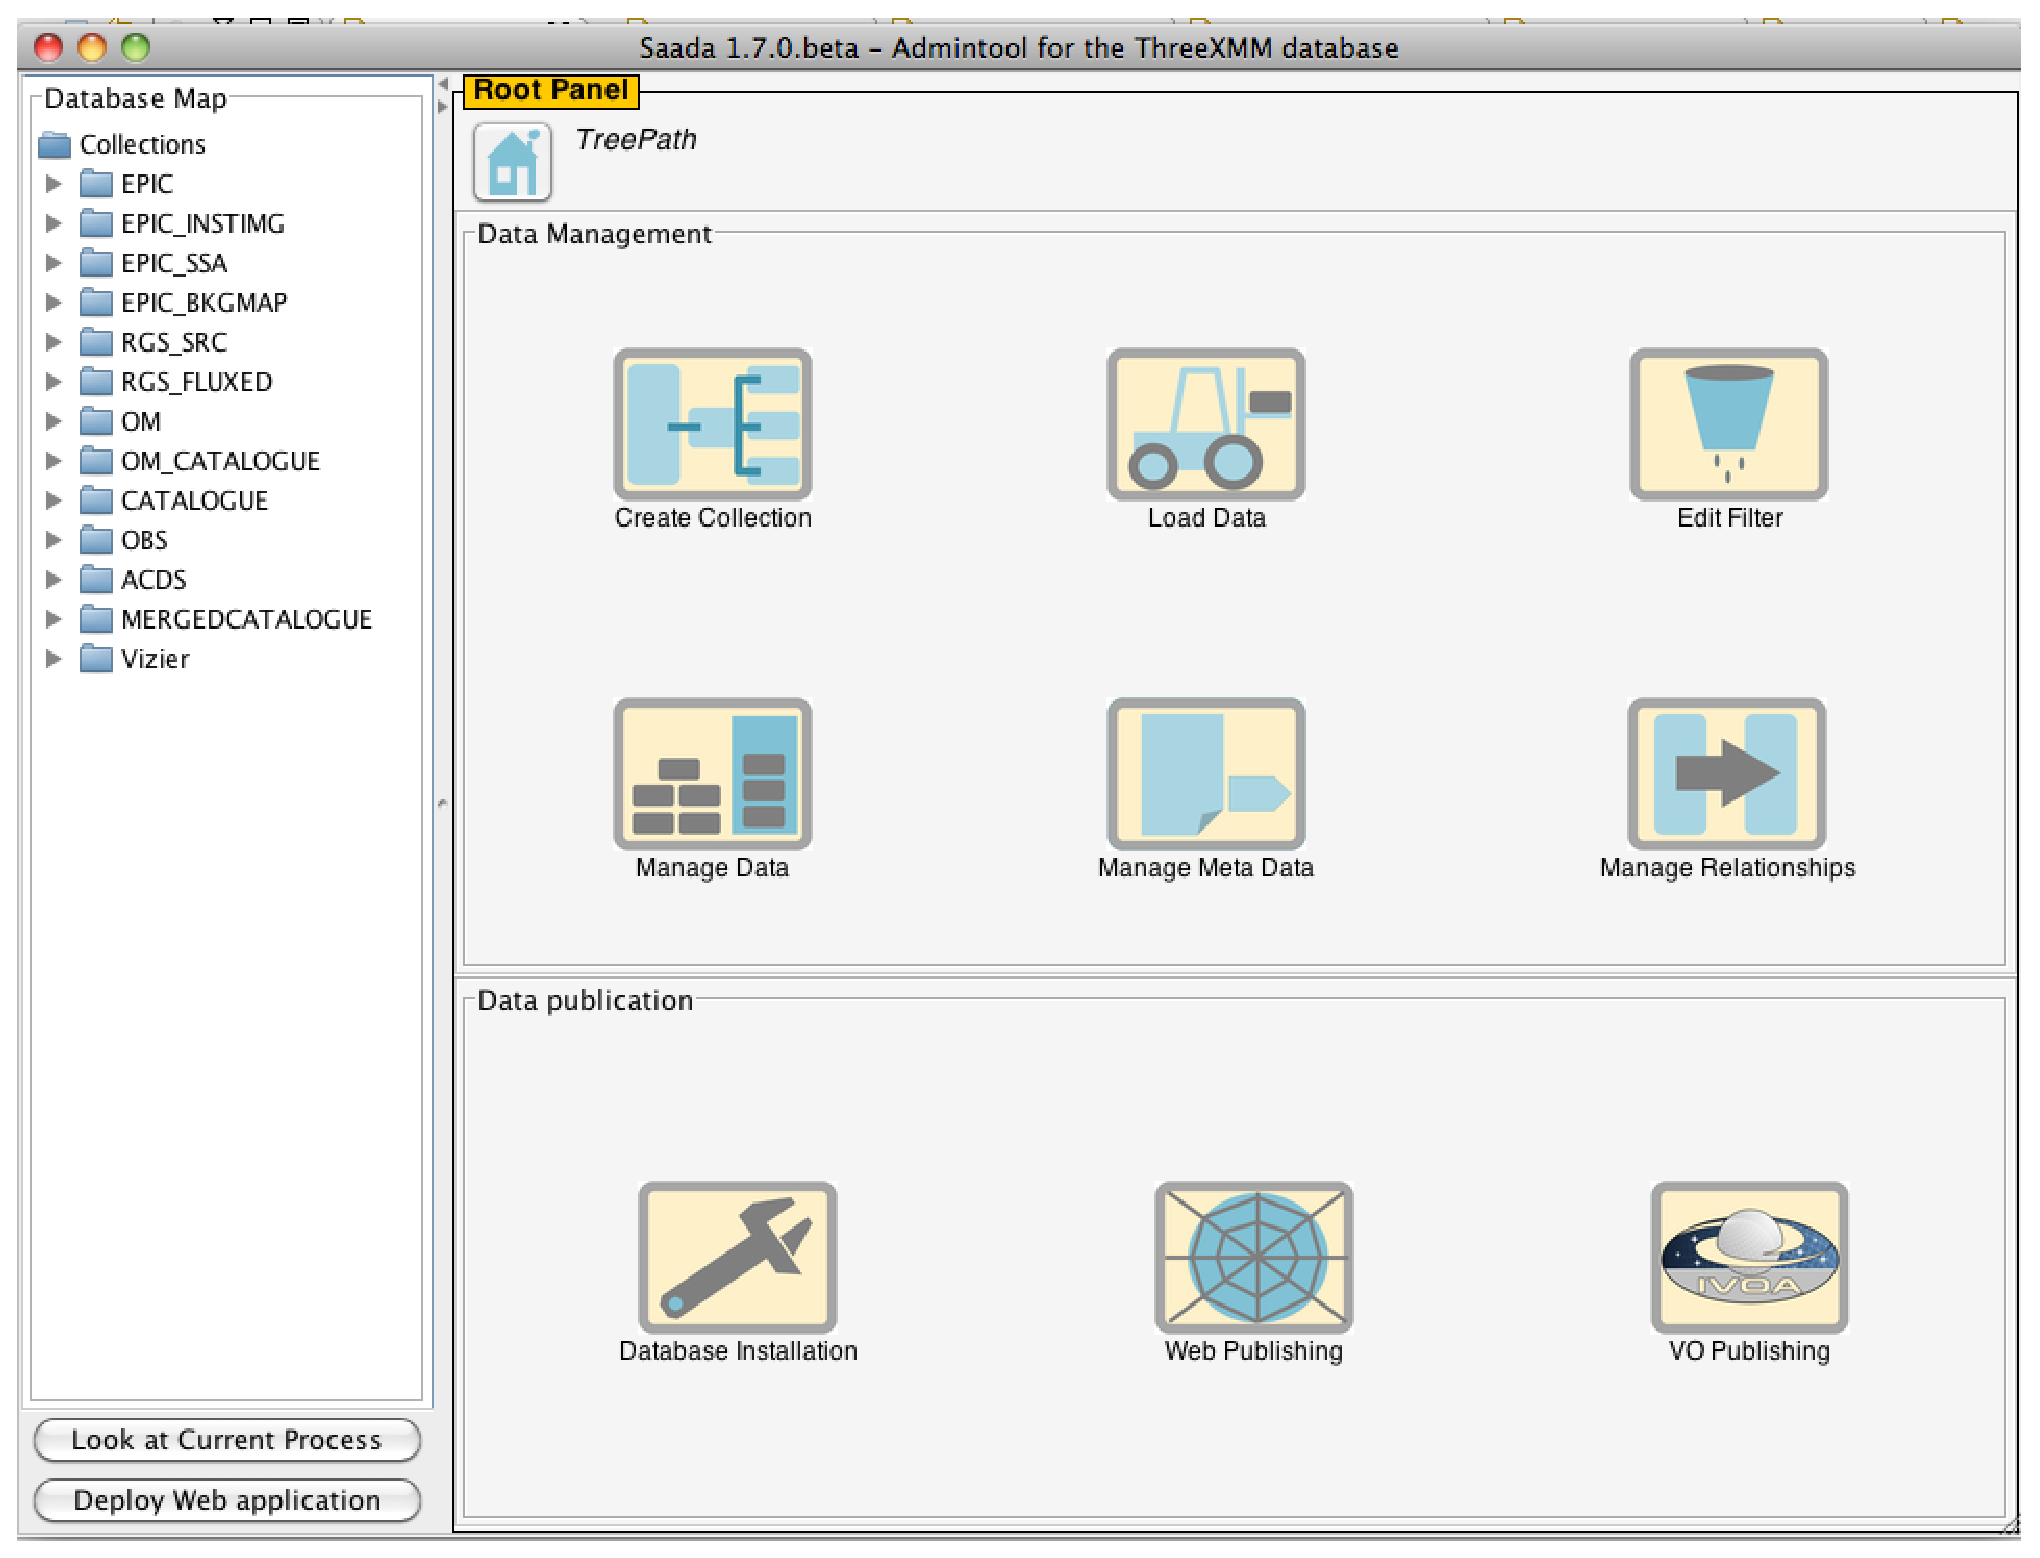
\includegraphics[width=0.70\textwidth]{part8/MICHEL_P18/P18_fig1.eps}
	\end{center}
	\caption{Welcome panel of the \ssindex{databases!tools!Saada}Saada\ooindex{Saada, ascl:1111.003} administration tool}
	\label{fig:fig1}
\end{figure}

\section{Ergonomics}
The tool is divided into three panels (Figure 1). The left panel shows a tree reflecting the database content. Selecting the data set on which an action must be performed is done by clicking on the corresponding node. A double click on a node opens a panel showing the node content. This panel includes an SQL editor allowing the user to refine data selection. The banner (Figure 2)  summarizes the current action (yellow frame) and the data node on which it is applied (blue label). It also contains two navigation buttons pointing to the previous panel and to the home panel. The right panel shows either a command panel or a set of icons opening further command panels. Each command panel has a footer bar with some action buttons (Figure 3). Possible actions are i) run the command ii) save the edited resource iii) switch the debug mode and iv) save the script file (see \S~4). Commands requiring a long execution time are handled by a distinct thread which can be controlled by a specific panel. This panel can be opened at any time with a button located below the data tree.

\begin{figure}[!ht]
	\begin{center}
		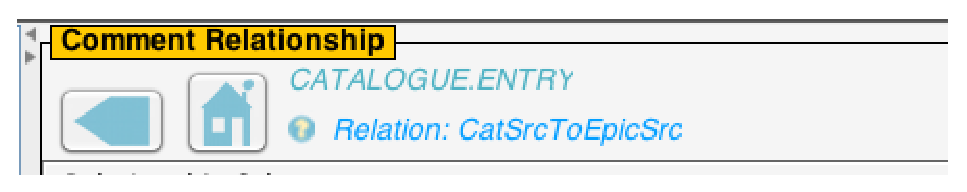
\includegraphics[height=0.10\textwidth]{part8/MICHEL_P18/P18_fig2.eps}
	\end{center}
	\caption{Banner summarizing the current action and the data node on which it is applied}
	\label{fig:fig2}
\end{figure}

\begin{figure}[!ht]
	\begin{center}
		
\includegraphics[height=0.10\textwidth]{part8/MICHEL_P18/P18_fig3.eps}
	\end{center}
	\caption{Action bar}
	\label{fig:fig3 (fig. 4)}
\end{figure}

\section{Data Management}
\begin{enumerate}
\item Data loading is done is two steps i) a loader filter must be edited first to map \ssindex{databases!tools!Saada}Saada\ooindex{Saada, ascl:1111.003} columns onto native columns or constant values. These filters are stored on disk and can be reused at any time. ii) data loading proper is achieved by a separated thread which can be interrupted by hand. This thread is transaction safe; the database remains consistent whatever are the conditions of its interruption.
\item Each entity (data classes, data collections and relationships) can receive a description to be reported on the Web interface or into \ssindex{data formats!VOTable}VOTables containing query results.
\item Relationships can be set between data collections. Links can be based on matching object positions on the sky or on any constraints on keywords or on both.\ssindex{databases!querylanguage!SQL} SQL templates are provided with the query editor.
\item Meta data (UCD, UTypes, units or descriptions) can be manually added to columns descriptions of ingested products. This meta data tagging is very important to make the database\ssindex{Virtual Observatory(VO)} VO compliant. Furthermore, the UCD/Unit pair can be used to build queries on heterogeneous data collections.
\end{enumerate}

\section{Script mode}
A novelty of this administration tool is the binding between the graphical mode and the script mode. Since the first releases, \ssindex{databases!tools!Saada}Saada\ooindex{Saada, ascl:1111.003} can be run in a script mode based on the \ssindex{software!tools!Ant}Ant utility\footnote{http://ant.apache.org}. This mode is very convenient for building a large or complex database in one shot. It also allows the management of a \ssindex{databases!tools!Saada}SaadaDB within a \ssindex{data!pipelines!reduction}pipeline \citep{P03_adassxxii}, however, the addition of\ssindex{software!tools!Ant} Ant configuration files is nonetheless painful. The new administration tool is now enabled to generate\ssindex{software!tools!Ant} Ant file reflecting the current action, which can thus be replayed in script mode. All steps of a complex database building can be developed separately in graphical mode on small data samples, and then the final database can be built in script mode by assembling all\ssindex{software!tools!Ant} Ant files.

\section{VO Publishing}
\ssindex{databases!tools!Saada}Saada\ooindex{Saada, ascl:1111.003} databases natively include three simple\ssindex{Virtual Observatory(VO)} VO services (\ssindex{protocols!SIAP}SIAP for images, \ssindex{protocols!SCS}SCS for catalogue entries and \ssindex{protocols!SSAP}SSAP for spectra \citep{SIAP,SCS,SSAP} ). Furthermore, \ssindex{databases!tools!Saada}Saada also supports both \ssindex{databases!querylanguage!ADQL}ADQL \citep{ADQL} and \ssindex{protocols!UWS}UWS \citep{UWS} which are the pillars of the\ssindex{Virtual Observatory(VO)} VO Table Access Protocol \citep{TAP}. In other words a \ssindex{databases!tools!Saada}SaadaDB is\ssindex{Virtual Observatory(VO)} VO ready, but publishing it in a registry \citep{REG} remains a bit difficult. Experience shows that it is more convenient to upload a valid \ssindex{data formats!XML}XML file in a public publishing registry than to use usual online forms. For each data collection, the administration tool can deliver a registry file ready to be uploaded. These files contain two parts i) the authority and curation part identifying the database itself and its owner. It is common for all published data collections. ii) the extension describing the published data set which is automatically generated according to the available meta data. The publication of a \ssindex{protocols!TAP}TAP service is somewhat less straightforward. The user must first select the\ssindex{databases!querylanguage!SQL} SQL tables he/she wants to publish, \ssindex{databases!tools!Saada}Saada\ooindex{Saada, ascl:1111.003} then automatically generates a \ssindex{protocols!TAP}TAP schema containing meta data for all tables. Any \ssindex{databases!tools!Saada}Saada\ooindex{Saada, ascl:1111.003} data collection can furthermore be mapped on an ObsCore view (Figure 4). ObsCore  is a simple generic data model used to perform data discovery when querying data centers for observations of interest \citep{OBSCORE}.

\begin{figure}[!h]
	\begin{center}
		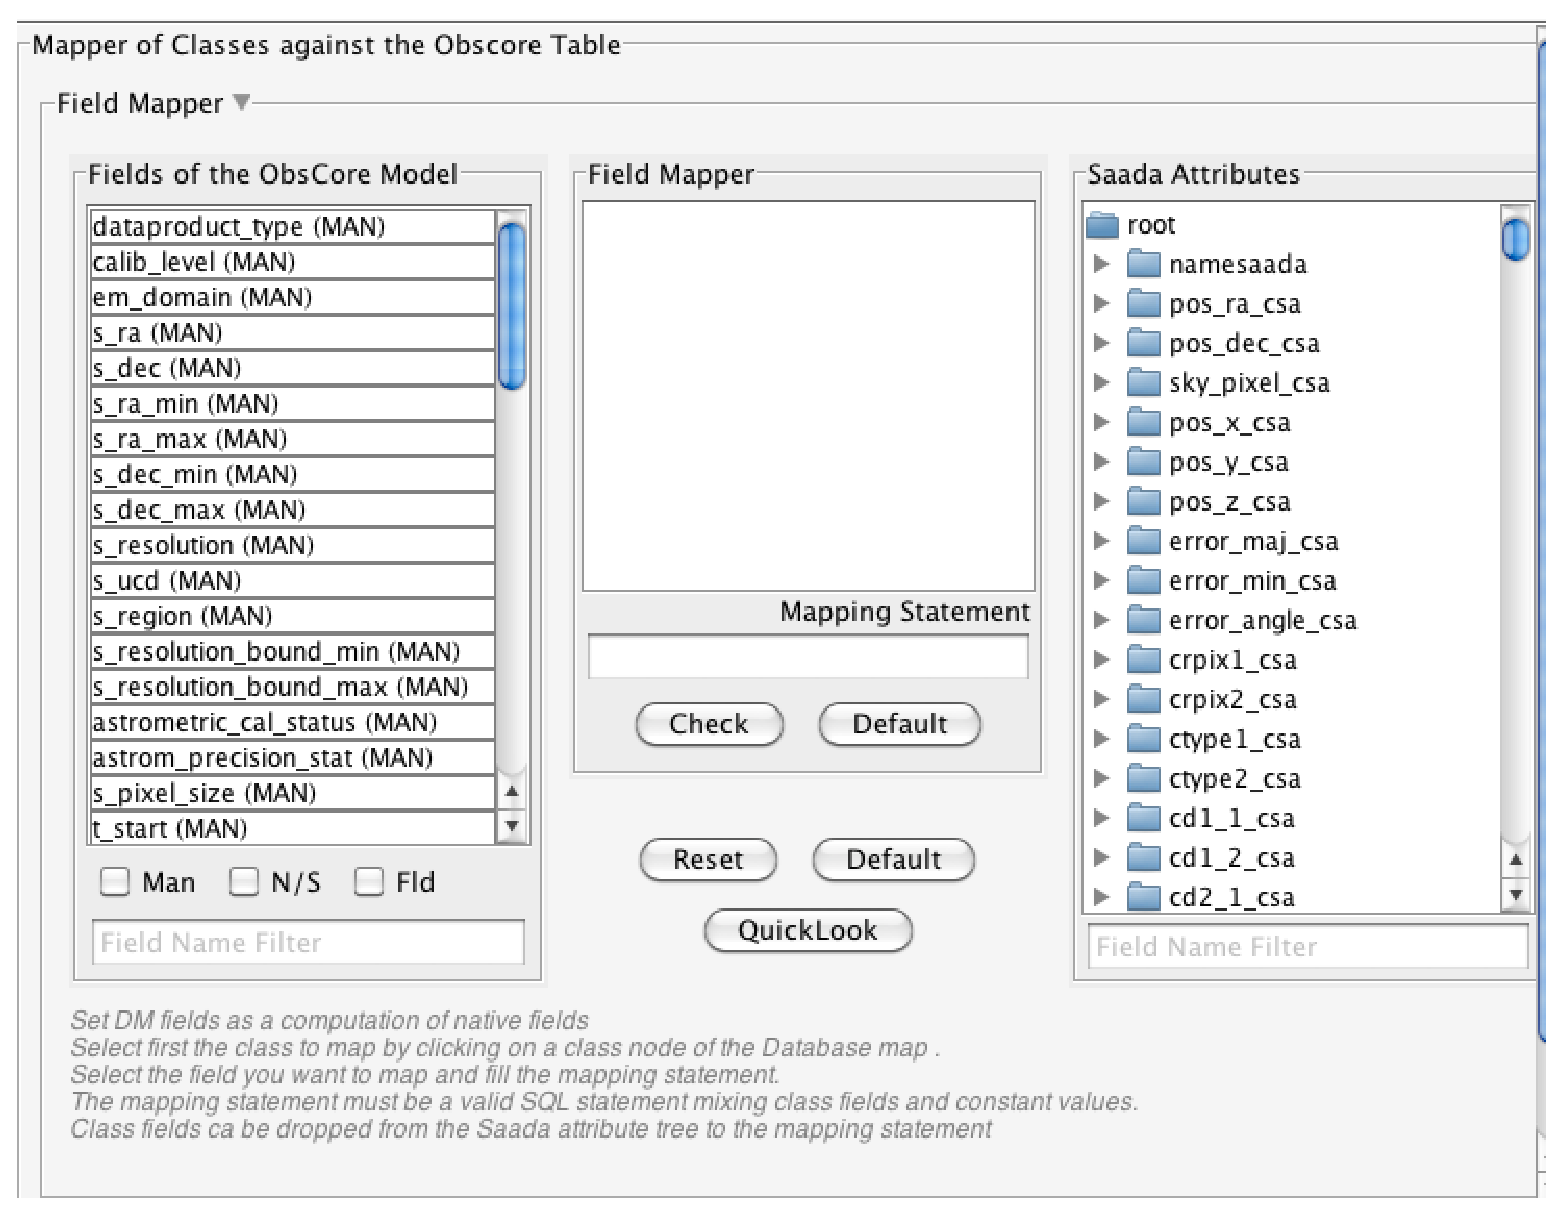
\includegraphics[width=0.60\textwidth]{part8/MICHEL_P18/P18_fig4.eps}
	\end{center}
	\caption{ObsCore mapper}
	\label{fig:fig4}
\end{figure}

\section {Conclusion and prospect}
This new interface will be officially released in the first quarter 2013. Upcoming \ssindex{databases!tools!Saada}Saada\ooindex{Saada, ascl:1111.003} version will adopt a major evolution of the inner data model in order to make \ssindex{databases!tools!Saada}Saada databases natively closer to\ssindex{Virtual Observatory(VO)} VO standards. Another development project targets the management of larger data collections.

\acknowledgements We would like to thank the \ssindex{observatories!space-based!XMM-Newton}XMM-Newton SSC team for supporting this project.

\bibliographystyle{asp2010}
\bibliography{editor}
